\documentclass{article}\usepackage[]{graphicx}\usepackage[]{color}
%% maxwidth is the original width if it is less than linewidth
%% otherwise use linewidth (to make sure the graphics do not exceed the margin)
\makeatletter
\def\maxwidth{ %
  \ifdim\Gin@nat@width>\linewidth
    \linewidth
  \else
    \Gin@nat@width
  \fi
}
\makeatother

\definecolor{fgcolor}{rgb}{0.345, 0.345, 0.345}
\newcommand{\hlnum}[1]{\textcolor[rgb]{0.686,0.059,0.569}{#1}}%
\newcommand{\hlstr}[1]{\textcolor[rgb]{0.192,0.494,0.8}{#1}}%
\newcommand{\hlcom}[1]{\textcolor[rgb]{0.678,0.584,0.686}{\textit{#1}}}%
\newcommand{\hlopt}[1]{\textcolor[rgb]{0,0,0}{#1}}%
\newcommand{\hlstd}[1]{\textcolor[rgb]{0.345,0.345,0.345}{#1}}%
\newcommand{\hlkwa}[1]{\textcolor[rgb]{0.161,0.373,0.58}{\textbf{#1}}}%
\newcommand{\hlkwb}[1]{\textcolor[rgb]{0.69,0.353,0.396}{#1}}%
\newcommand{\hlkwc}[1]{\textcolor[rgb]{0.333,0.667,0.333}{#1}}%
\newcommand{\hlkwd}[1]{\textcolor[rgb]{0.737,0.353,0.396}{\textbf{#1}}}%

\usepackage{framed}
\makeatletter
\newenvironment{kframe}{%
 \def\at@end@of@kframe{}%
 \ifinner\ifhmode%
  \def\at@end@of@kframe{\end{minipage}}%
  \begin{minipage}{\columnwidth}%
 \fi\fi%
 \def\FrameCommand##1{\hskip\@totalleftmargin \hskip-\fboxsep
 \colorbox{shadecolor}{##1}\hskip-\fboxsep
     % There is no \\@totalrightmargin, so:
     \hskip-\linewidth \hskip-\@totalleftmargin \hskip\columnwidth}%
 \MakeFramed {\advance\hsize-\width
   \@totalleftmargin\z@ \linewidth\hsize
   \@setminipage}}%
 {\par\unskip\endMakeFramed%
 \at@end@of@kframe}
\makeatother

\definecolor{shadecolor}{rgb}{.97, .97, .97}
\definecolor{messagecolor}{rgb}{0, 0, 0}
\definecolor{warningcolor}{rgb}{1, 0, 1}
\definecolor{errorcolor}{rgb}{1, 0, 0}
\newenvironment{knitrout}{}{} % an empty environment to be redefined in TeX

\usepackage{alltt}
\usepackage{fullpage}
\usepackage{placeins}
\usepackage[colorlinks=true, linkcolor=blue]{hyperref}
\title{Lab 3 Pattern Analysis-Hypothesis Testing}
\author{Dominic LaRoche}
\IfFileExists{upquote.sty}{\usepackage{upquote}}{}
\begin{document}
\maketitle

\section{Assigment I}
Based on the inclusion of simulation results (fig.~\ref{fest}) we can conclude that the japanese pine sapling data is not different from complete spatial randomness (CSR).
\begin{knitrout}
\definecolor{shadecolor}{rgb}{0.969, 0.969, 0.969}\color{fgcolor}\begin{kframe}
\begin{alltt}
\hlkwd{rm}\hlstd{(}\hlkwc{list}\hlstd{=}\hlkwd{ls}\hlstd{())}
\hlkwd{library}\hlstd{(spatstat)}
\end{alltt}


{\ttfamily\noindent\itshape\color{messagecolor}{\#\# \\\#\# spatstat 1.38-1\ \ \ \ \ \  (nickname: 'Le Hardi') \\\#\# For an introduction to spatstat, type 'beginner'}}\begin{alltt}
\hlkwd{data}\hlstd{(japanesepines)}
\hlstd{jp}\hlkwb{<-}\hlstd{japanesepines}
\end{alltt}
\end{kframe}
\end{knitrout}








\begin{figure}
\begin{knitrout}
\definecolor{shadecolor}{rgb}{0.969, 0.969, 0.969}\color{fgcolor}\begin{kframe}
\begin{alltt}
\hlstd{fhat.env}\hlkwb{<-}\hlkwa{function}\hlstd{(}\hlkwc{n}\hlstd{,} \hlkwc{s}\hlstd{,} \hlkwc{r}\hlstd{,} \hlkwc{win}\hlstd{=}\hlkwd{owin}\hlstd{(}\hlkwd{c}\hlstd{(}\hlnum{0}\hlstd{,}\hlnum{1}\hlstd{),}\hlkwd{c}\hlstd{(}\hlnum{0}\hlstd{,}\hlnum{1}\hlstd{)))\{}
  \hlcom{#function to create upper and lower CSR bounds on Fest}
  \hlstd{hold}\hlkwb{<-}\hlkwd{matrix}\hlstd{(}\hlnum{0}\hlstd{,s,} \hlkwd{length}\hlstd{(r))}
  \hlkwa{for} \hlstd{(i} \hlkwa{in} \hlnum{1}\hlopt{:}\hlstd{s)\{}
    \hlstd{hold[i,]}\hlkwb{<-}\hlkwd{Fest}\hlstd{(}\hlkwd{runifpoint}\hlstd{(n,}\hlkwc{win}\hlstd{=win),} \hlkwc{r}\hlstd{=r)}\hlopt{$}\hlstd{rs}
  \hlstd{\}}
  \hlstd{mn}\hlkwb{<-}\hlkwd{apply}\hlstd{(hold,} \hlnum{2}\hlstd{, mean)}
  \hlstd{Up}\hlkwb{<-}\hlkwd{apply}\hlstd{(hold,}\hlnum{2}\hlstd{,max)}
  \hlstd{Down}\hlkwb{<-}\hlkwd{apply}\hlstd{(hold,}\hlnum{2}\hlstd{,min)}
  \hlkwd{return}\hlstd{(}\hlkwd{data.frame}\hlstd{(mn,Up, Down))}
\hlstd{\}}

\hlstd{jp.fhat}\hlkwb{<-}\hlkwd{Fest}\hlstd{(jp)}
\hlstd{jp.win}\hlkwb{<-}\hlkwd{window}\hlstd{(jp)}
\hlkwd{plot}\hlstd{(jp.fhat, rs}\hlopt{~}\hlstd{r,} \hlkwc{main}\hlstd{=}\hlstr{"F estimates"}\hlstd{)}
\hlstd{jp.fenv}\hlkwb{<-}\hlkwd{fhat.env}\hlstd{(}\hlkwc{n}\hlstd{=jp}\hlopt{$}\hlstd{n,} \hlkwc{s}\hlstd{=}\hlnum{100}\hlstd{,} \hlkwc{r}\hlstd{=jp.fhat}\hlopt{$}\hlstd{r,} \hlkwc{win}\hlstd{=jp.win)}
\hlcom{#upper and lower envelopes}
\hlkwd{lines}\hlstd{(jp.fhat}\hlopt{$}\hlstd{r, jp.fenv}\hlopt{$}\hlstd{Up,}\hlkwc{lty}\hlstd{=}\hlnum{5}\hlstd{,} \hlkwc{col}\hlstd{=}\hlnum{2}\hlstd{)}
\hlkwd{lines}\hlstd{(jp.fhat}\hlopt{$}\hlstd{r,jp.fenv}\hlopt{$}\hlstd{Down,}\hlkwc{lty}\hlstd{=}\hlnum{5}\hlstd{,} \hlkwc{col}\hlstd{=}\hlnum{2}\hlstd{)}
\end{alltt}
\end{kframe}
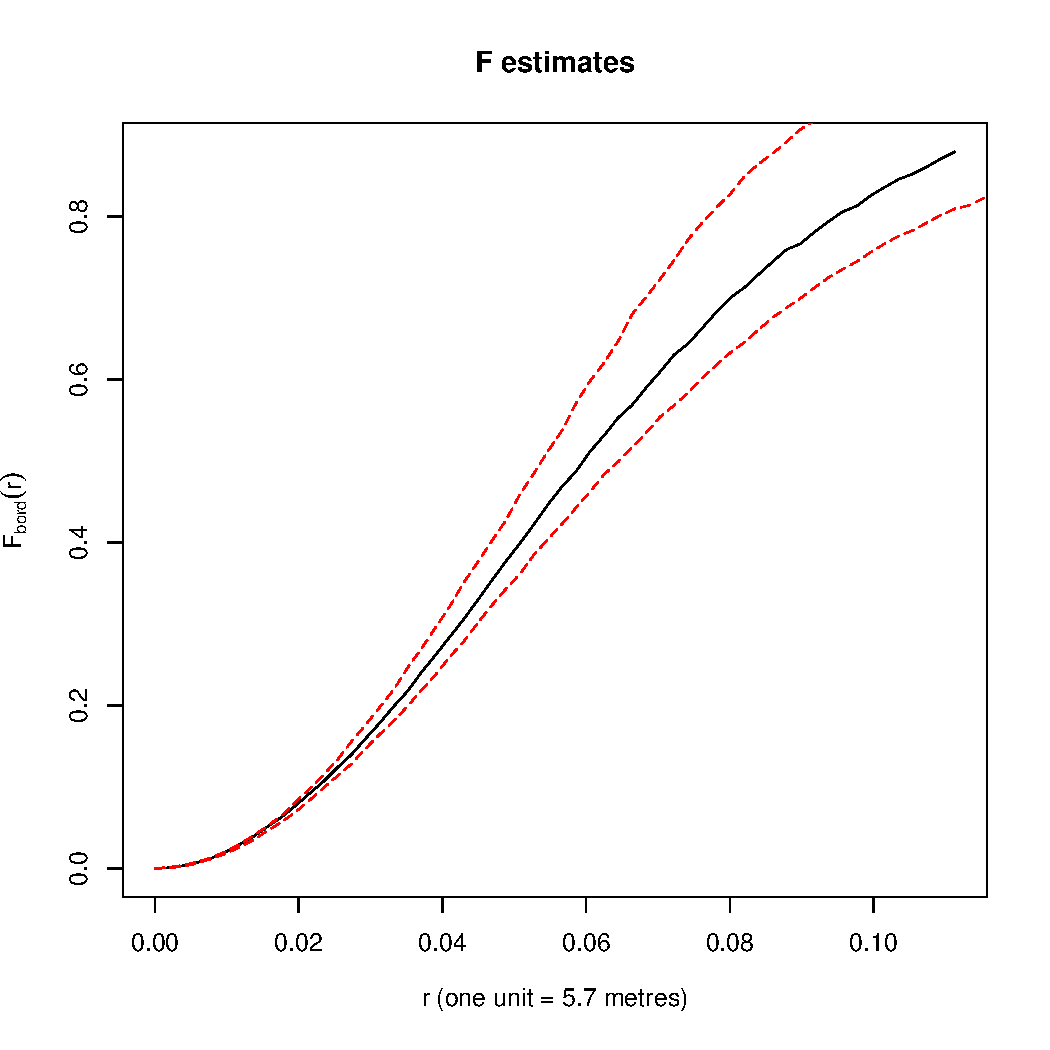
\includegraphics[width=\maxwidth]{figure/FestBounds} 

\end{knitrout}
\caption{Plot of $\hat{F}$ with upper and lower envelopes simulated from completely spatially random (CSR) data.}
\label{fest}
\end{figure}

\FloatBarrier

\section{Assignment II}
Here I define a function to get upper and lower bounds for the K function:\\
\begin{knitrout}
\definecolor{shadecolor}{rgb}{0.969, 0.969, 0.969}\color{fgcolor}\begin{kframe}
\begin{alltt}
\hlstd{khat.env}\hlkwb{<-}\hlkwa{function}\hlstd{(}\hlkwc{n}\hlstd{,} \hlkwc{s}\hlstd{,} \hlkwc{r}\hlstd{,} \hlkwc{win}\hlstd{=}\hlkwd{owin}\hlstd{(}\hlkwd{c}\hlstd{(}\hlnum{0}\hlstd{,}\hlnum{1}\hlstd{),}\hlkwd{c}\hlstd{(}\hlnum{0}\hlstd{,}\hlnum{1}\hlstd{)))\{}
  \hlcom{#function to create upper and lower CSR bounds on Fest}
  \hlstd{hold}\hlkwb{<-}\hlkwd{matrix}\hlstd{(}\hlnum{0}\hlstd{,s,} \hlkwd{length}\hlstd{(r))}
  \hlkwa{for} \hlstd{(i} \hlkwa{in} \hlnum{1}\hlopt{:}\hlstd{s)\{}
    \hlstd{hold[i,]}\hlkwb{<-}\hlkwd{Kest}\hlstd{(}\hlkwd{runifpoint}\hlstd{(n,}\hlkwc{win}\hlstd{=win),} \hlkwc{r}\hlstd{=r)}\hlopt{$}\hlstd{border}
  \hlstd{\}}
  \hlstd{mn}\hlkwb{<-}\hlkwd{apply}\hlstd{(hold,} \hlnum{2}\hlstd{, mean)}
  \hlstd{Up}\hlkwb{<-}\hlkwd{apply}\hlstd{(hold,}\hlnum{2}\hlstd{,max)}
  \hlstd{Down}\hlkwb{<-}\hlkwd{apply}\hlstd{(hold,}\hlnum{2}\hlstd{,min)}
  \hlkwd{return}\hlstd{(}\hlkwd{data.frame}\hlstd{(mn,Up, Down))}
\hlstd{\}}
\end{alltt}
\end{kframe}
\end{knitrout}
Based on the plot of the K-function with upper and lower bounds created from simulated CSR data (fig.~\ref{kest}), we can conclude that the Japanese pine saplings are not significantly different from CSR.\\

\begin{figure}
\begin{knitrout}
\definecolor{shadecolor}{rgb}{0.969, 0.969, 0.969}\color{fgcolor}\begin{kframe}
\begin{alltt}
\hlstd{jp.khat}\hlkwb{<-}\hlkwd{Kest}\hlstd{(jp)}
\hlkwd{plot}\hlstd{(jp.khat,} \hlkwd{cbind}\hlstd{(border, theo)}\hlopt{~}\hlstd{r,} \hlkwc{main}\hlstd{=}\hlstr{"K function for JP data"}\hlstd{)}
\end{alltt}
\begin{verbatim}
##        lty col    key           label                           meaning
## border   1   1 border hat(K)[bord](r) border-corrected estimate of K(r)
## theo     2   2   theo      K[pois](r)          theoretical Poisson K(r)
\end{verbatim}
\begin{alltt}
\hlstd{jp.kenv}\hlkwb{<-}\hlkwd{khat.env}\hlstd{(}\hlkwc{n}\hlstd{=jp}\hlopt{$}\hlstd{n,} \hlkwc{s}\hlstd{=}\hlnum{100}\hlstd{,} \hlkwc{r}\hlstd{=jp.khat}\hlopt{$}\hlstd{r,} \hlkwc{win}\hlstd{=jp.win)}
\hlcom{#upper and lower envelopes}
\hlkwd{lines}\hlstd{(jp.khat}\hlopt{$}\hlstd{r, jp.kenv}\hlopt{$}\hlstd{Up,}\hlkwc{lty}\hlstd{=}\hlnum{5}\hlstd{,} \hlkwc{col}\hlstd{=}\hlnum{3}\hlstd{)}
\hlkwd{lines}\hlstd{(jp.khat}\hlopt{$}\hlstd{r,jp.kenv}\hlopt{$}\hlstd{Down,}\hlkwc{lty}\hlstd{=}\hlnum{5}\hlstd{,} \hlkwc{col}\hlstd{=}\hlnum{3}\hlstd{)}
\end{alltt}
\end{kframe}
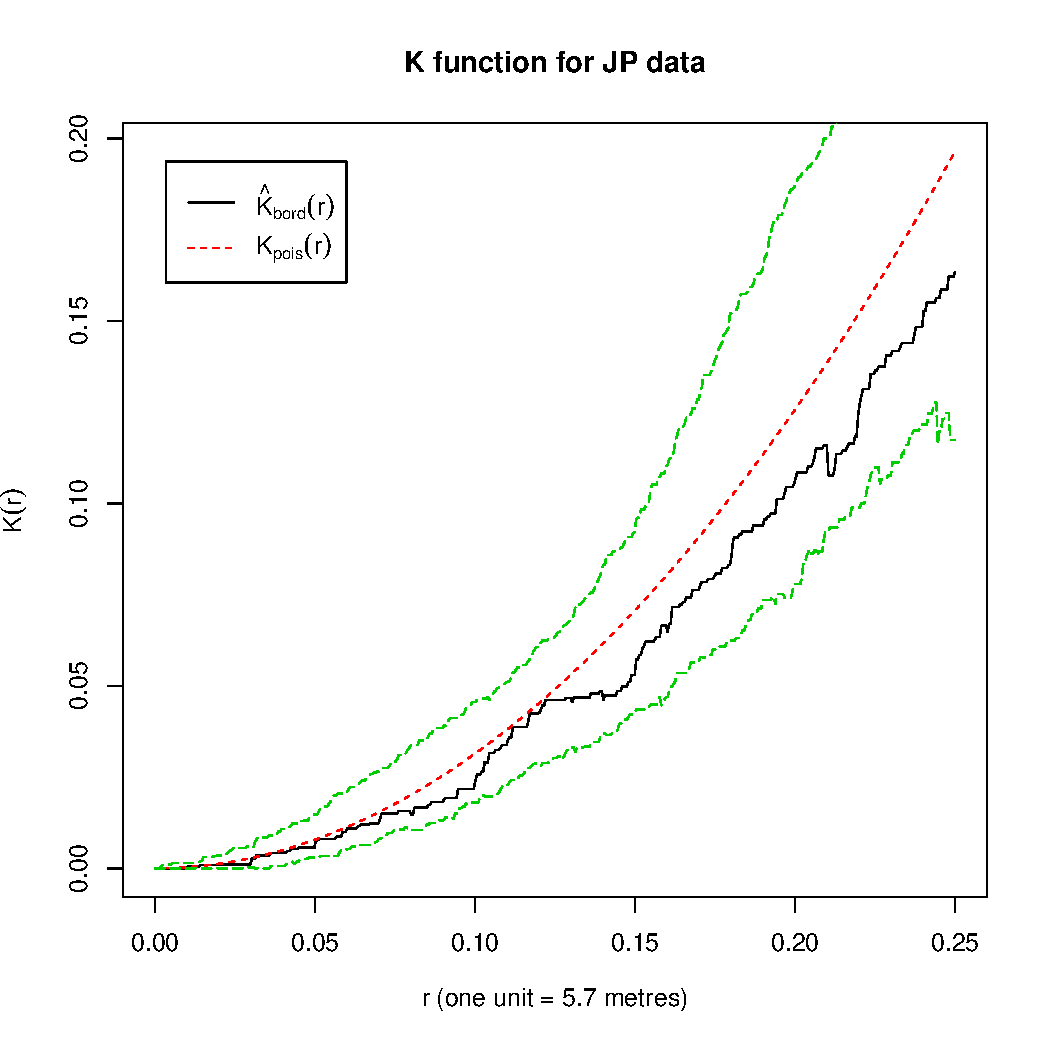
\includegraphics[width=\maxwidth]{figure/Kboundplot} 

\end{knitrout}
\caption{Plot of the $\hat{K}$ function with upper  and lower bounds created from simulated CSR data.  The red dashed line represents the theoretical K-function for a poisson CSR pattern.}
\label{kest}
\end{figure}

\FloatBarrier

\section{Assignment III}

\begin{knitrout}
\definecolor{shadecolor}{rgb}{0.969, 0.969, 0.969}\color{fgcolor}\begin{kframe}
\begin{alltt}
\hlkwd{data}\hlstd{(redwood)} \hlcom{#load the dataset}
\hlcom{# summary(redwood)}
\hlstd{regular}\hlkwb{<-}\hlkwd{rsyst}\hlstd{(}\hlkwc{nx}\hlstd{=}\hlnum{10}\hlstd{)} \hlcom{#generate regular pattern}
\hlcom{# summary(regular)}
\hlstd{rdwd}\hlkwb{<-}\hlstd{redwood}
\end{alltt}
\end{kframe}
\end{knitrout}

\subsection{Quadrat Tests}
We will test for a first order effect using two different quadrat tests, one with 4 cells (2x2) and one with 16 (4x4).  The two grids are shown in figure~\ref{quads}.\\

\begin{figure}
\begin{knitrout}
\definecolor{shadecolor}{rgb}{0.969, 0.969, 0.969}\color{fgcolor}\begin{kframe}
\begin{alltt}
\hlkwd{par}\hlstd{(}\hlkwc{mfrow}\hlstd{=}\hlkwd{c}\hlstd{(}\hlnum{1}\hlstd{,}\hlnum{2}\hlstd{))}
\hlcom{#2x2}
\hlstd{q.rdwd2}\hlkwb{<-}\hlkwd{quadratcount}\hlstd{(rdwd,}\hlkwc{nx}\hlstd{=}\hlnum{2}\hlstd{,}\hlkwc{ny}\hlstd{=}\hlnum{2}\hlstd{)}
\hlkwd{plot} \hlstd{(rdwd,} \hlkwc{pch}\hlstd{=}\hlstr{"+"}\hlstd{,} \hlkwc{main} \hlstd{=} \hlstr{" 2x2 Quadrat for redwood data"}\hlstd{)}
\hlkwd{plot} \hlstd{(q.rdwd2,} \hlkwc{add}\hlstd{=}\hlnum{TRUE}\hlstd{,} \hlkwc{col}\hlstd{=}\hlstr{"red"}\hlstd{,} \hlkwc{cex}\hlstd{=}\hlnum{1.5}\hlstd{,} \hlkwc{lty}\hlstd{=}\hlnum{2}\hlstd{)}
\hlcom{#4x4}
\hlstd{q.rdwd4}\hlkwb{<-}\hlkwd{quadratcount}\hlstd{(rdwd,}\hlkwc{nx}\hlstd{=}\hlnum{4}\hlstd{,}\hlkwc{ny}\hlstd{=}\hlnum{4}\hlstd{)}
\hlkwd{plot} \hlstd{(rdwd,} \hlkwc{pch}\hlstd{=}\hlstr{"+"}\hlstd{,} \hlkwc{main} \hlstd{=} \hlstr{"4x4 Quadrat for rdwd data"}\hlstd{)}
\hlkwd{plot} \hlstd{(q.rdwd4,} \hlkwc{add}\hlstd{=}\hlnum{TRUE}\hlstd{,} \hlkwc{col}\hlstd{=}\hlstr{"red"}\hlstd{,} \hlkwc{cex}\hlstd{=}\hlnum{1.5}\hlstd{,} \hlkwc{lty}\hlstd{=}\hlnum{2}\hlstd{)}
\end{alltt}
\end{kframe}
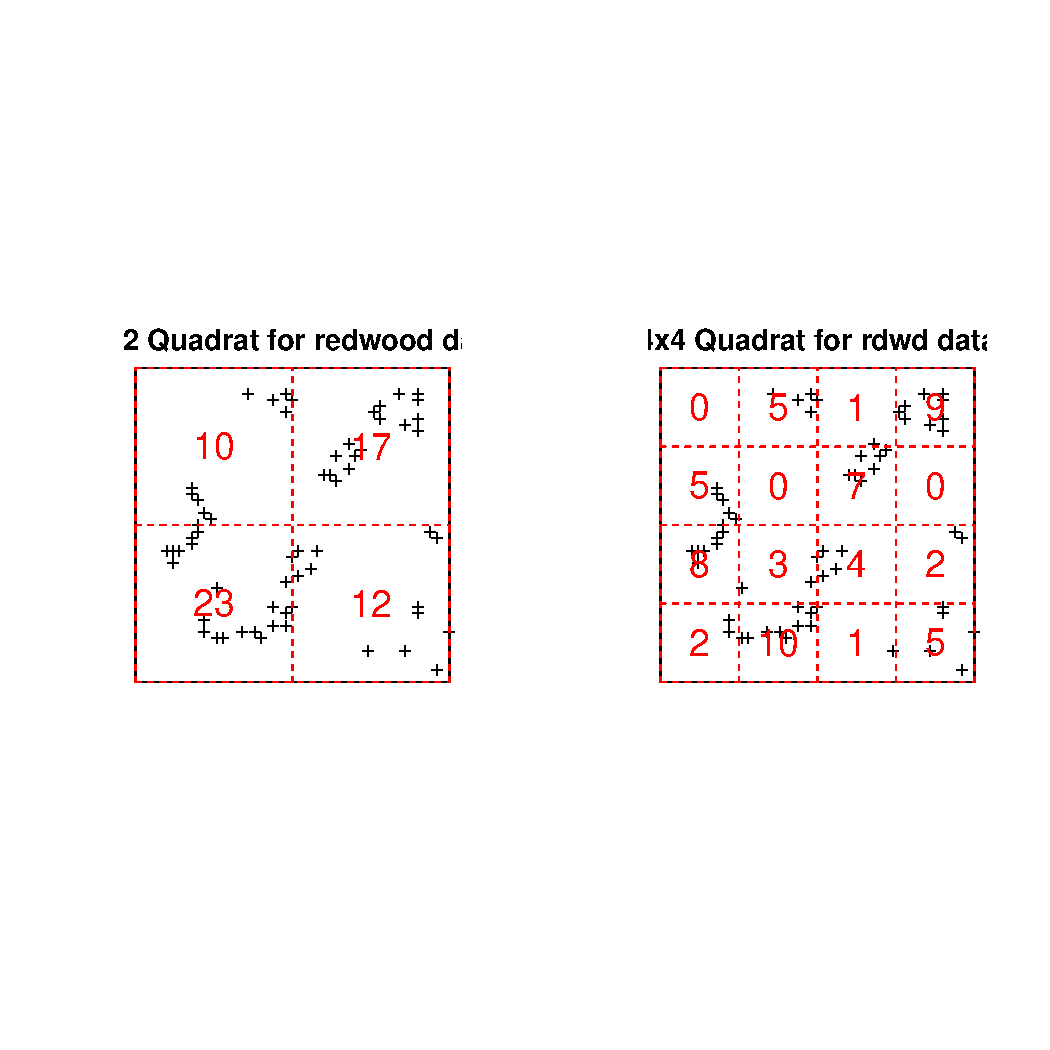
\includegraphics[width=\maxwidth]{figure/FirstOrderEffect} 

\end{knitrout}
\caption{Quadrat counts for the California redwood data.}
\label{quads}
\end{figure}

We cannot reject the null hypothesis of complete spatial randomness with the 2x2 quadrat tests ($\alpha \geq 0.1$).  However, the 4x4 quadrat test produced a highly significant result (p-value = 0.0004). Figures ~\ref{qt.rdwd2} and ~\ref{qt.rdwd4} show the counts and expected values for each cell.\\
\begin{knitrout}
\definecolor{shadecolor}{rgb}{0.969, 0.969, 0.969}\color{fgcolor}\begin{kframe}
\begin{alltt}
\hlstd{qt.rdwd2}\hlkwb{<-}\hlkwd{quadrat.test}\hlstd{(rdwd,}\hlnum{2}\hlstd{,}\hlnum{2}\hlstd{)}
\hlstd{qt.rdwd2}
\end{alltt}
\begin{verbatim}
## 
## 	Chi-squared test of CSR using quadrat counts
## 	Pearson X2 statistic
## 
## data:  rdwd
## X2 = 6.516, df = 3, p-value = 0.1781
## alternative hypothesis: two.sided
## 
## Quadrats: 2 by 2 grid of tiles
\end{verbatim}
\begin{alltt}
\hlstd{qt.rdwd4}\hlkwb{<-}\hlkwd{quadrat.test}\hlstd{(rdwd,}\hlnum{4}\hlstd{,}\hlnum{4}\hlstd{)}
\end{alltt}


{\ttfamily\noindent\color{warningcolor}{\#\# Warning: Some expected counts are small; chi\textasciicircum{}2 approximation may be inaccurate}}\begin{alltt}
\hlstd{qt.rdwd4}
\end{alltt}
\begin{verbatim}
## 
## 	Chi-squared test of CSR using quadrat counts
## 	Pearson X2 statistic
## 
## data:  rdwd
## X2 = 42.26, df = 15, p-value = 0.0004102
## alternative hypothesis: two.sided
## 
## Quadrats: 4 by 4 grid of tiles
\end{verbatim}
\end{kframe}
\end{knitrout}

\begin{figure}
\begin{knitrout}
\definecolor{shadecolor}{rgb}{0.969, 0.969, 0.969}\color{fgcolor}\begin{kframe}
\begin{alltt}
\hlkwd{plot}\hlstd{(qt.rdwd2,} \hlkwc{main}\hlstd{=}\hlstr{"Quadrat Test: 2x2 rdwd data"}\hlstd{)}
\hlkwd{plot}\hlstd{(rdwd,} \hlkwc{pch}\hlstd{=}\hlstr{"+"}\hlstd{,} \hlkwc{col}\hlstd{=}\hlstr{"red"}\hlstd{,} \hlkwc{add}\hlstd{=T)}
\end{alltt}
\end{kframe}
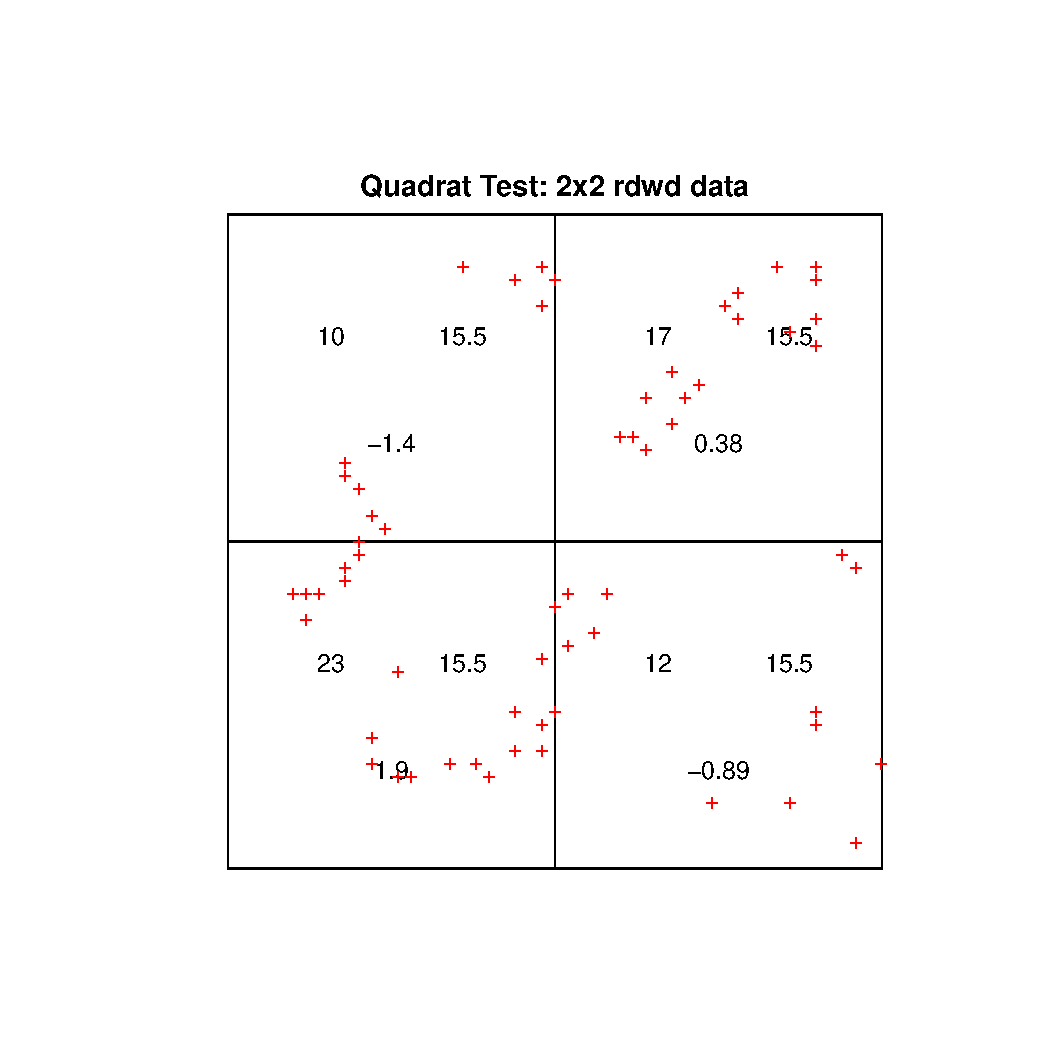
\includegraphics[width=\maxwidth]{figure/plottests2x2} 

\end{knitrout}
\caption{A plot of the test for the 2x2 quadrat test.}
\label{qt.rdwd2}
\end{figure}

\begin{figure}
\begin{knitrout}
\definecolor{shadecolor}{rgb}{0.969, 0.969, 0.969}\color{fgcolor}\begin{kframe}
\begin{alltt}
\hlkwd{plot}\hlstd{(qt.rdwd4,} \hlkwc{main}\hlstd{=}\hlstr{"Quadrat Test: 4x4 rdwd data"}\hlstd{)}
\hlkwd{plot}\hlstd{(rdwd,} \hlkwc{pch}\hlstd{=}\hlstr{"+"}\hlstd{,} \hlkwc{col}\hlstd{=}\hlstr{"red"}\hlstd{,} \hlkwc{add}\hlstd{=T)}
\end{alltt}
\end{kframe}
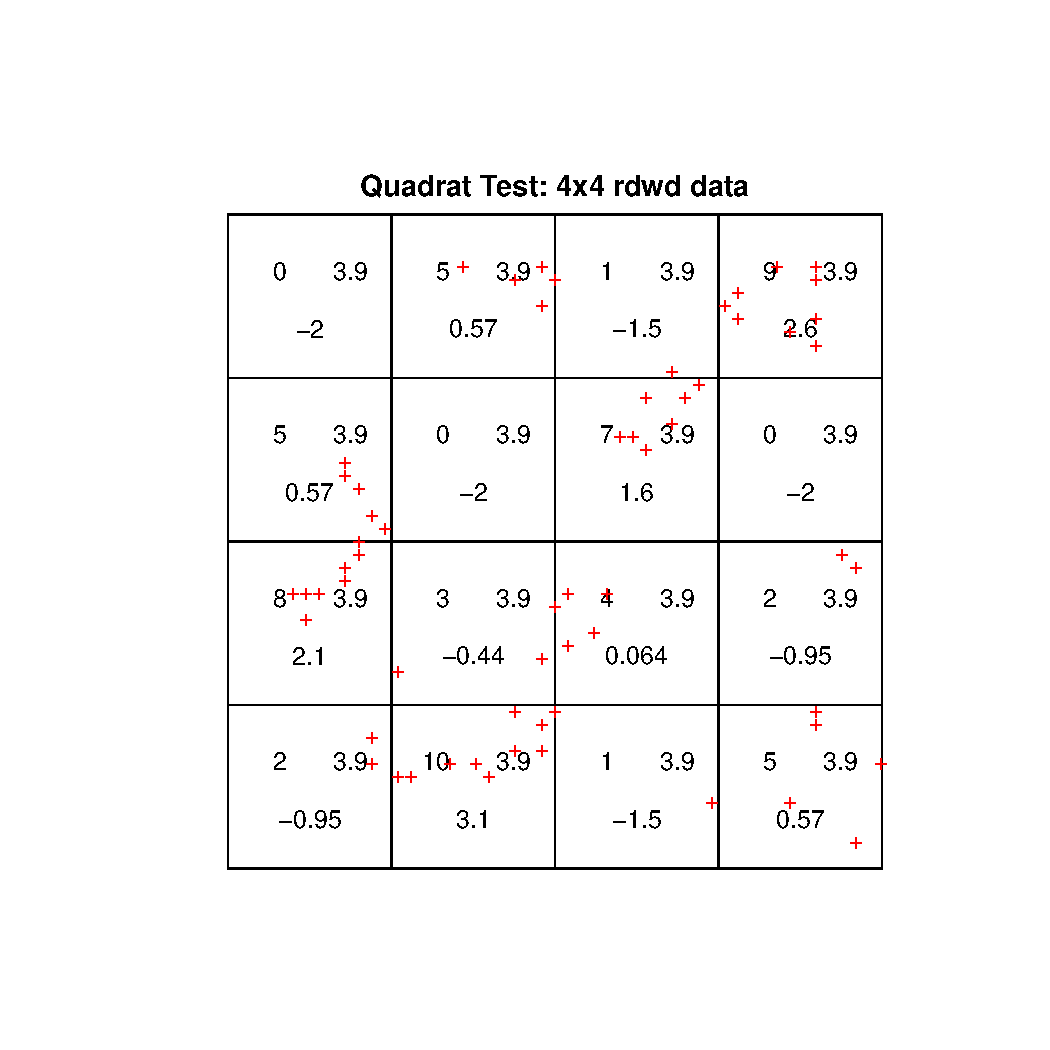
\includegraphics[width=\maxwidth]{figure/plottests4x4} 

\end{knitrout}
\caption{A plot of the test for the 4x4 quadrat test.}
\label{qt.rdwd4}
\end{figure}
\FloatBarrier

\subsection{Kernel estimation}
Figure~\ref{kern} shows two different realizations of kernel density estimation with bandwidths equal to 0.05 (top) and 0.1 (bottom) for both the Japanese pine sapling data and the California redwood data.  Both bandwidth values appear to indicate clustering of the points in the redwood data (bottom) whereas the pine data (top) is not as well captured by either kernel.\\
\begin{figure}
\begin{knitrout}
\definecolor{shadecolor}{rgb}{0.969, 0.969, 0.969}\color{fgcolor}\begin{kframe}
\begin{alltt}
\hlcom{# ?density.ppp}
\hlkwd{par}\hlstd{(}\hlkwc{mfrow}\hlstd{=}\hlkwd{c}\hlstd{(}\hlnum{2}\hlstd{,}\hlnum{2}\hlstd{))}
\hlstd{jp.Z.0.5}\hlkwb{<-}\hlkwd{density.ppp}\hlstd{(jp,} \hlnum{0.05}\hlstd{)}
\hlkwd{plot}\hlstd{(jp.Z.0.5,} \hlkwc{main}\hlstd{=}\hlstr{"JP: sigma=0.05"}\hlstd{)}
\hlkwd{points}\hlstd{(jp,} \hlkwc{pch}\hlstd{=}\hlstr{"+"}\hlstd{,} \hlkwc{col}\hlstd{=}\hlstr{"6"}\hlstd{)}

\hlstd{jp.Z.1}\hlkwb{<-}\hlkwd{density.ppp}\hlstd{(jp,} \hlnum{0.1}\hlstd{)}
\hlkwd{plot}\hlstd{(jp.Z.1,} \hlkwc{main}\hlstd{=}\hlstr{"JP: sigma =0.1"}\hlstd{)}
\hlkwd{points}\hlstd{(jp,} \hlkwc{pch}\hlstd{=}\hlstr{"+"}\hlstd{,} \hlkwc{col}\hlstd{=}\hlstr{"6"}\hlstd{)}

\hlstd{rdwd.Z.0.5}\hlkwb{<-}\hlkwd{density.ppp}\hlstd{(rdwd,} \hlnum{0.05}\hlstd{)}
\hlkwd{plot}\hlstd{(rdwd.Z.0.5,} \hlkwc{main}\hlstd{=}\hlstr{"RdWd: Sigma=0.05"}\hlstd{)}
\hlkwd{points}\hlstd{(rdwd,} \hlkwc{pch}\hlstd{=}\hlstr{"+"}\hlstd{,} \hlkwc{col}\hlstd{=}\hlstr{"6"}\hlstd{)}

\hlstd{rdwd.Z.1}\hlkwb{<-}\hlkwd{density.ppp}\hlstd{(rdwd,} \hlnum{0.1}\hlstd{)}
\hlkwd{plot}\hlstd{(rdwd.Z.1,} \hlkwc{main}\hlstd{=}\hlstr{"RdWd: Sigma =0.1"}\hlstd{)}
\hlkwd{points}\hlstd{(rdwd,} \hlkwc{pch}\hlstd{=}\hlstr{"+"}\hlstd{,} \hlkwc{col}\hlstd{=}\hlstr{"6"}\hlstd{)}
\end{alltt}
\end{kframe}
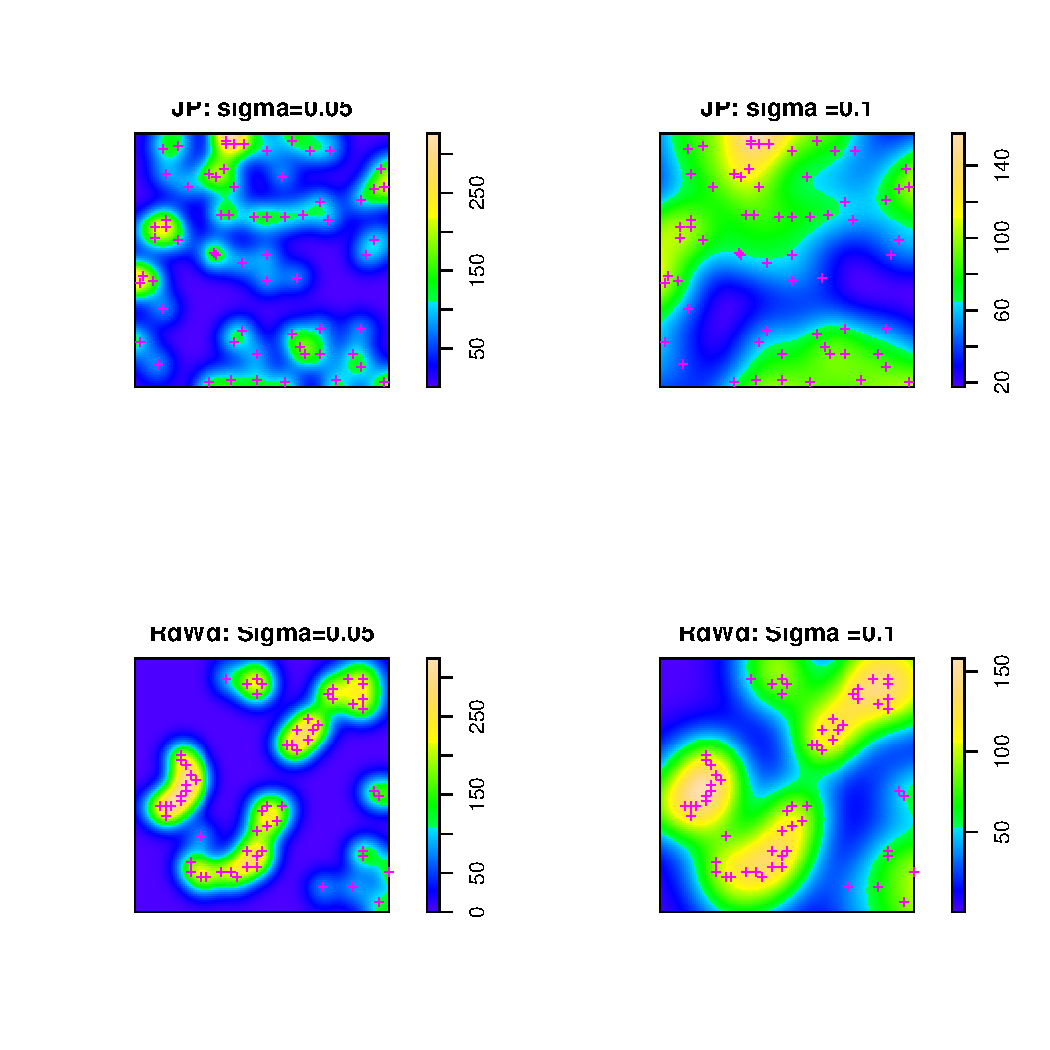
\includegraphics[width=\maxwidth]{figure/kernelest05} 

\end{knitrout}
\caption{Two different kernel density estimation with sigma =0.05 and 0.1 for the Japanese pine sapling data (top) and the redwood data (bottom).}
\label{kern}
\end{figure}
\FloatBarrier

\subsection{Second Order Effect}
The plots of $\hat{G}$ (fig.~\ref{gest2}) and $\hat{F}$ (fig.~\ref{fest2}) both suggest that the pattern is not random for the California redwood data.  In the $\hat{G}$ plot the ECDF lies above the upper and lower bounds generated from simulated CSR data.  This suggests that the redwood saplings are clustered in space. The same inference is made from the $\hat{F}$ plot in which the distance between a random point and an observed point is larger than one would expect with CSR points.  The $\hat{K}$ function plot (fig.~\ref{kest2}) and the $\hat{L}$ function both  Also indicate clustering in the California redwood data.  For all plots references above the Japanese pine sapling data lies within the CSR bounds calculated from simulated CSR data.  This indicates that we cannot reject the null hypothesis of CSR.\\

\begin{figure}
\begin{knitrout}
\definecolor{shadecolor}{rgb}{0.969, 0.969, 0.969}\color{fgcolor}\begin{kframe}
\begin{alltt}
\hlstd{rdwd.ghat}\hlkwb{<-}\hlkwd{Gest}\hlstd{(rdwd)}
\hlstd{rdwd.win}\hlkwb{<-}\hlkwd{window}\hlstd{(rdwd)}
\hlkwd{plot}\hlstd{(rdwd.ghat, rs}\hlopt{~}\hlstd{r,} \hlkwc{main}\hlstd{=}\hlstr{"G estimates"}\hlstd{)}
\hlkwd{plot}\hlstd{(jp.ghat, rs}\hlopt{~}\hlstd{r,} \hlkwc{add}\hlstd{=T,} \hlkwc{col}\hlstd{=}\hlnum{4}\hlstd{)}

\hlstd{rdwd.genv}\hlkwb{<-}\hlkwd{ghat.env}\hlstd{(}\hlkwc{n}\hlstd{=rdwd}\hlopt{$}\hlstd{n,} \hlkwc{s}\hlstd{=}\hlnum{100}\hlstd{,} \hlkwc{r}\hlstd{=rdwd.ghat}\hlopt{$}\hlstd{r,} \hlkwc{win}\hlstd{=rdwd.win)}
\hlcom{#upper and lower envelopes}
\hlkwd{lines}\hlstd{(rdwd.ghat}\hlopt{$}\hlstd{r, rdwd.genv}\hlopt{$}\hlstd{Up,}\hlkwc{lty}\hlstd{=}\hlnum{5}\hlstd{,} \hlkwc{col}\hlstd{=}\hlnum{2}\hlstd{)}
\hlkwd{lines}\hlstd{(rdwd.ghat}\hlopt{$}\hlstd{r,rdwd.genv}\hlopt{$}\hlstd{Down,}\hlkwc{lty}\hlstd{=}\hlnum{5}\hlstd{,} \hlkwc{col}\hlstd{=}\hlnum{2}\hlstd{)}
\hlkwd{legend}\hlstd{(}\hlstr{"topleft"}\hlstd{,}\hlkwc{legend}\hlstd{=}\hlkwd{c}\hlstd{(}\hlstr{"Redwood"}\hlstd{,}\hlstr{"Pine"}\hlstd{,}\hlstr{"CSR Bounds"}\hlstd{),}\hlkwc{col}\hlstd{=}\hlkwd{c}\hlstd{(}\hlnum{1}\hlstd{,}\hlnum{4}\hlstd{,}\hlnum{2}\hlstd{),}\hlkwc{lty}\hlstd{=}\hlkwd{c}\hlstd{(}\hlnum{1}\hlstd{,}\hlnum{1}\hlstd{,}\hlnum{5}\hlstd{))}
\end{alltt}
\end{kframe}
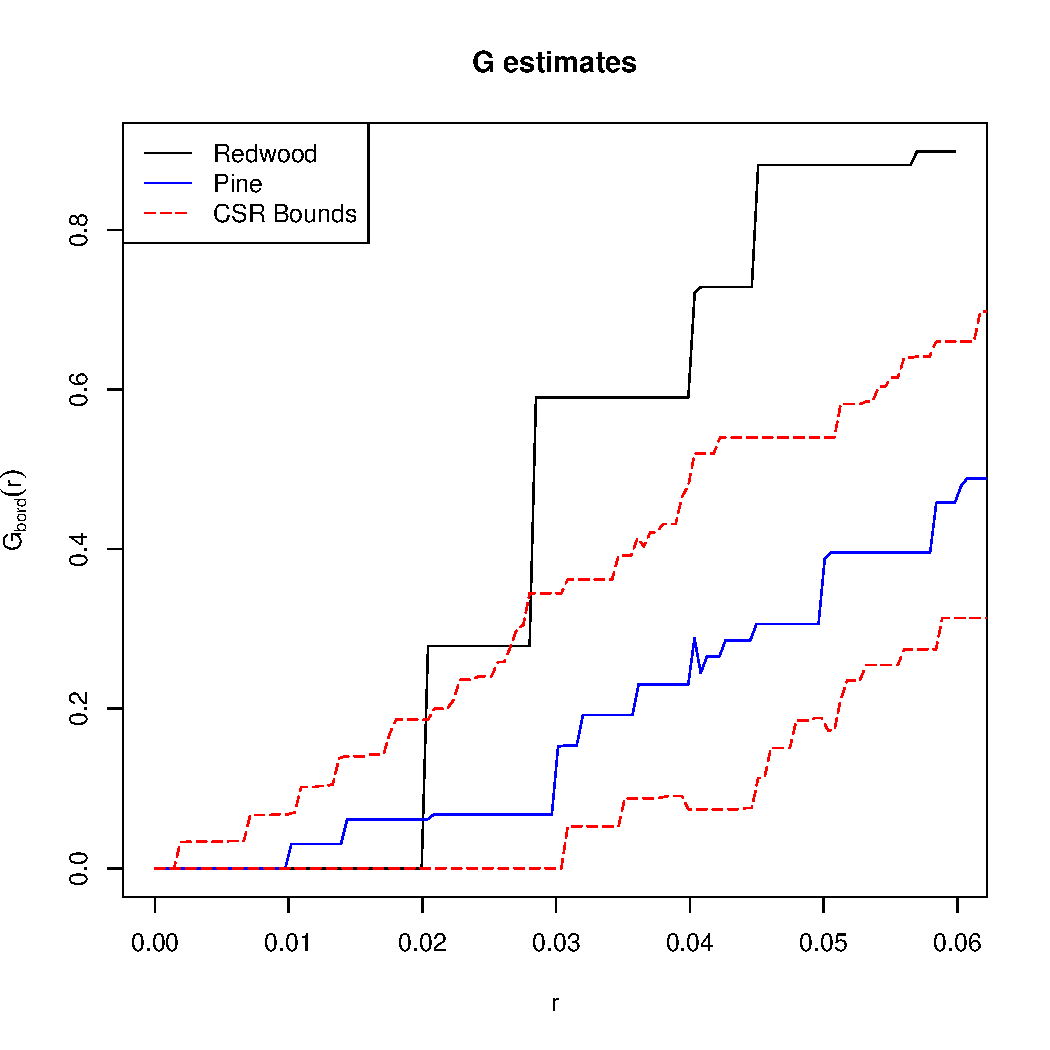
\includegraphics[width=\maxwidth]{figure/secondorder} 

\end{knitrout}
\caption{Estimation of the G function using nearest neighbor distances and comparison with simulated upper and lower bounds of poisson CSR data.  The black line represents the redwood data and falls outside the CSR bounds whereas the blue line represents the Japanese pine data and falls inside the CSR bounds}
\label{gest2}
\end{figure}

\begin{figure}
\begin{knitrout}
\definecolor{shadecolor}{rgb}{0.969, 0.969, 0.969}\color{fgcolor}\begin{kframe}
\begin{alltt}
\hlstd{rdwd.fhat}\hlkwb{<-}\hlkwd{Fest}\hlstd{(rdwd)}
\hlkwd{plot}\hlstd{(rdwd.fhat, rs}\hlopt{~}\hlstd{r,} \hlkwc{main}\hlstd{=}\hlstr{"F estimates"}\hlstd{)}
\hlkwd{plot}\hlstd{(jp.fhat, rs}\hlopt{~}\hlstd{r,} \hlkwc{add}\hlstd{=T,} \hlkwc{col}\hlstd{=}\hlnum{4}\hlstd{)}
\hlstd{rdwd.fenv}\hlkwb{<-}\hlkwd{fhat.env}\hlstd{(}\hlkwc{n}\hlstd{=rdwd}\hlopt{$}\hlstd{n,} \hlkwc{s}\hlstd{=}\hlnum{100}\hlstd{,} \hlkwc{r}\hlstd{=rdwd.fhat}\hlopt{$}\hlstd{r,} \hlkwc{win}\hlstd{=rdwd.win)}
\hlcom{#upper and lower envelopes}
\hlkwd{lines}\hlstd{(rdwd.fhat}\hlopt{$}\hlstd{r, rdwd.fenv}\hlopt{$}\hlstd{Up,}\hlkwc{lty}\hlstd{=}\hlnum{5}\hlstd{,} \hlkwc{col}\hlstd{=}\hlnum{2}\hlstd{)}
\hlkwd{lines}\hlstd{(rdwd.fhat}\hlopt{$}\hlstd{r,rdwd.fenv}\hlopt{$}\hlstd{Down,}\hlkwc{lty}\hlstd{=}\hlnum{5}\hlstd{,} \hlkwc{col}\hlstd{=}\hlnum{2}\hlstd{)}
\hlkwd{legend}\hlstd{(}\hlstr{"topleft"}\hlstd{,}\hlkwc{legend}\hlstd{=}\hlkwd{c}\hlstd{(}\hlstr{"Redwood"}\hlstd{,}\hlstr{"Pine"}\hlstd{,}\hlstr{"CSR Bounds"}\hlstd{),}\hlkwc{col}\hlstd{=}\hlkwd{c}\hlstd{(}\hlnum{1}\hlstd{,}\hlnum{4}\hlstd{,}\hlnum{2}\hlstd{),}\hlkwc{lty}\hlstd{=}\hlkwd{c}\hlstd{(}\hlnum{1}\hlstd{,}\hlnum{1}\hlstd{,}\hlnum{5}\hlstd{))}
\end{alltt}
\end{kframe}
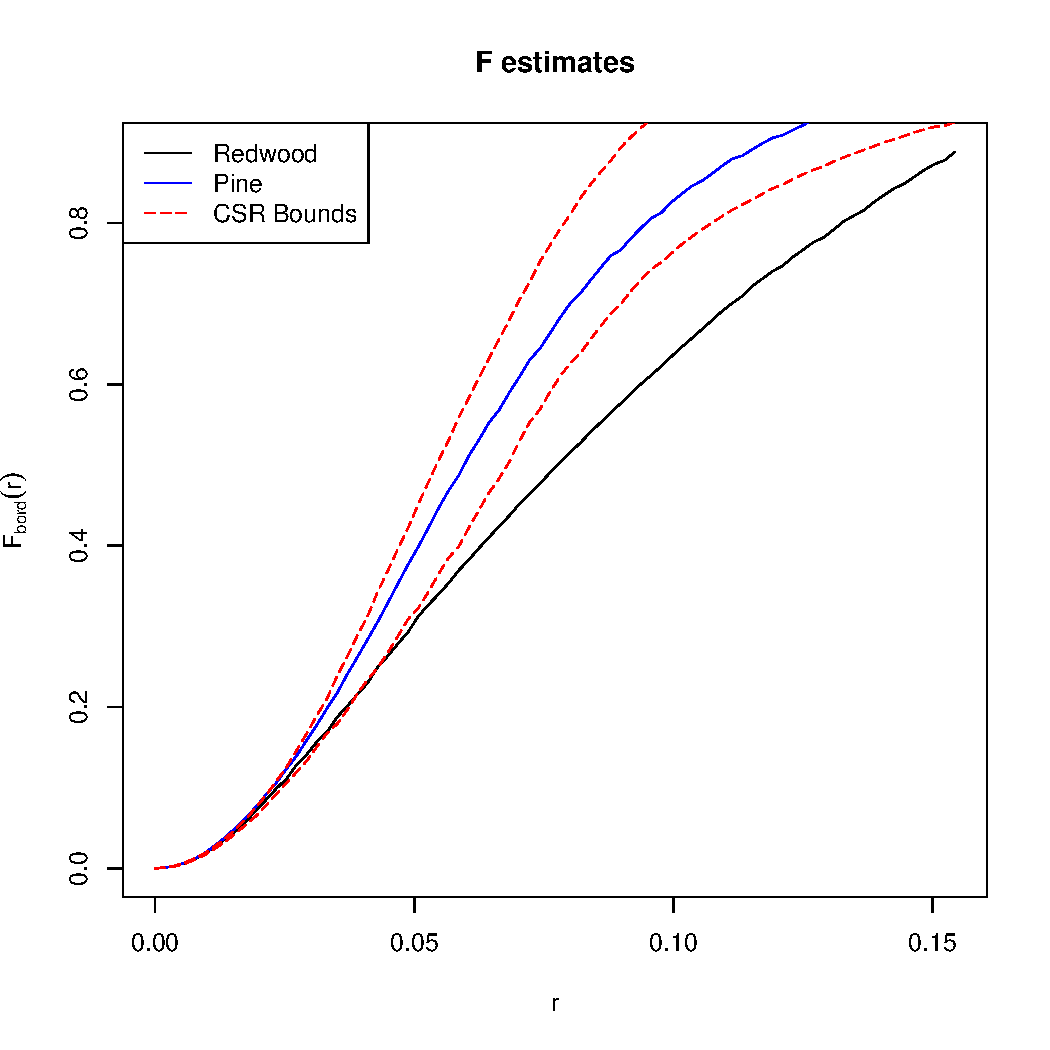
\includegraphics[width=\maxwidth]{figure/secondorder2} 

\end{knitrout}
\caption{Estimation of the F function using point-to-event distances and comparison with upper and lower bounds generated from CSR data for both the Japanese pine sapling data and the California redwood data.  As before the redwood data lies outside the CSR bounds whereas the pine data lies inside.}
\label{fest2}
\end{figure}

\begin{figure}
\begin{knitrout}
\definecolor{shadecolor}{rgb}{0.969, 0.969, 0.969}\color{fgcolor}\begin{kframe}
\begin{alltt}
\hlstd{rdwd.khat}\hlkwb{<-}\hlkwd{Kest}\hlstd{(rdwd)}
\hlkwd{plot}\hlstd{(rdwd.khat, border}\hlopt{~}\hlstd{r,} \hlkwc{main}\hlstd{=}\hlstr{"K function for rdwd data"}\hlstd{)}
\hlkwd{plot}\hlstd{(jp.khat, border}\hlopt{~}\hlstd{r,} \hlkwc{add}\hlstd{=T,} \hlkwc{col}\hlstd{=}\hlnum{4}\hlstd{)}
\hlstd{rdwd.kenv}\hlkwb{<-}\hlkwd{khat.env}\hlstd{(}\hlkwc{n}\hlstd{=rdwd}\hlopt{$}\hlstd{n,} \hlkwc{s}\hlstd{=}\hlnum{100}\hlstd{,} \hlkwc{r}\hlstd{=rdwd.khat}\hlopt{$}\hlstd{r,} \hlkwc{win}\hlstd{=rdwd.win)}
\hlcom{#upper and lower envelopes}
\hlkwd{lines}\hlstd{(rdwd.khat}\hlopt{$}\hlstd{r, rdwd.kenv}\hlopt{$}\hlstd{Up,}\hlkwc{lty}\hlstd{=}\hlnum{5}\hlstd{,} \hlkwc{col}\hlstd{=}\hlnum{2}\hlstd{)}
\hlkwd{lines}\hlstd{(rdwd.khat}\hlopt{$}\hlstd{r,rdwd.kenv}\hlopt{$}\hlstd{Down,}\hlkwc{lty}\hlstd{=}\hlnum{5}\hlstd{,} \hlkwc{col}\hlstd{=}\hlnum{2}\hlstd{)}
\hlkwd{legend}\hlstd{(}\hlstr{"topleft"}\hlstd{,}\hlkwc{legend}\hlstd{=}\hlkwd{c}\hlstd{(}\hlstr{"Redwood"}\hlstd{,}\hlstr{"Pine"}\hlstd{,}\hlstr{"CSR Bounds"}\hlstd{),}\hlkwc{col}\hlstd{=}\hlkwd{c}\hlstd{(}\hlnum{1}\hlstd{,}\hlnum{4}\hlstd{,}\hlnum{2}\hlstd{),}\hlkwc{lty}\hlstd{=}\hlkwd{c}\hlstd{(}\hlnum{1}\hlstd{,}\hlnum{1}\hlstd{,}\hlnum{5}\hlstd{))}
\end{alltt}
\end{kframe}
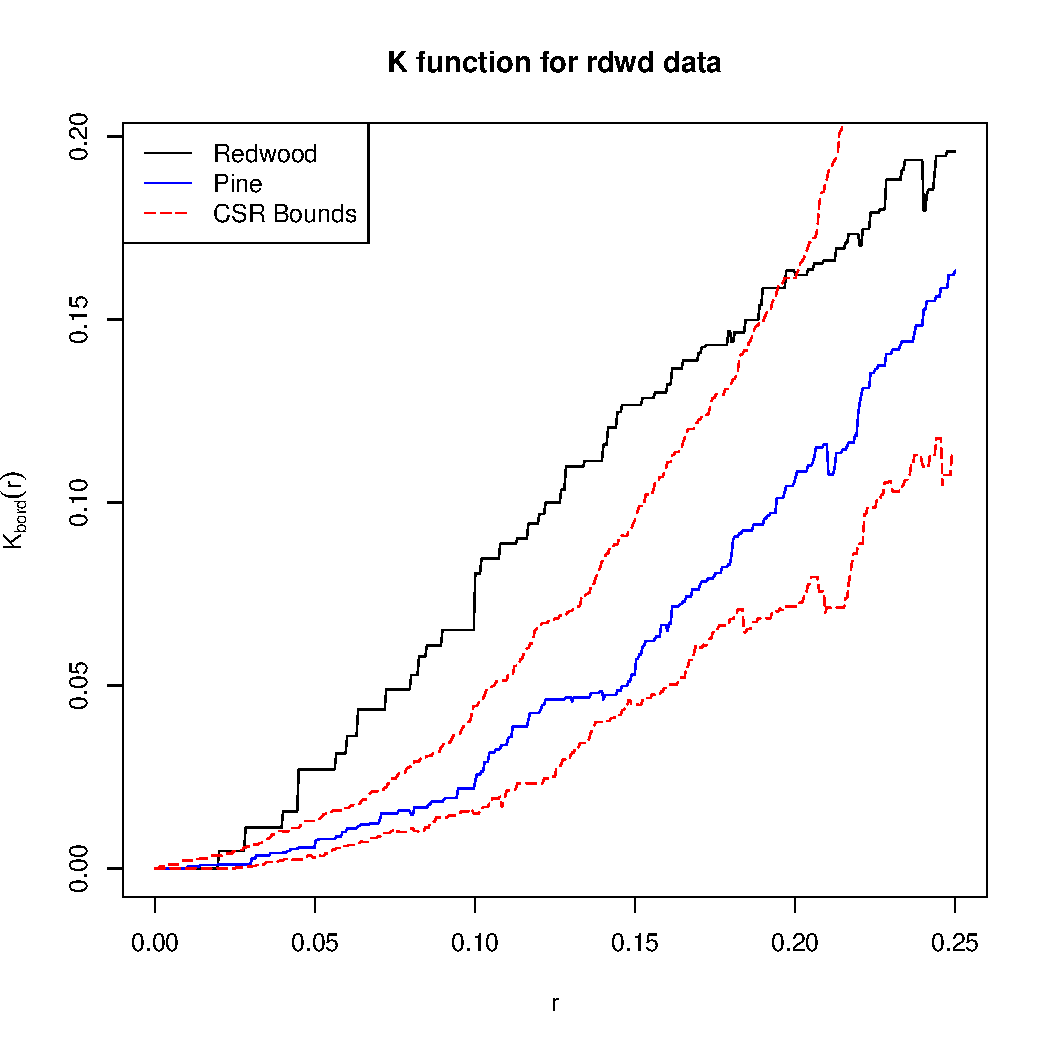
\includegraphics[width=\maxwidth]{figure/Kest} 

\end{knitrout}
\caption{Plot of the K function for the redwood data showing the same pattern as the $\hat{G}$ and $\hat{F}$ plots, i.e. the redwood data appears clustered and the pine data lies within what we would expect from CSR data.}
\label{kest2}
\end{figure}

\begin{figure}
\begin{knitrout}
\definecolor{shadecolor}{rgb}{0.969, 0.969, 0.969}\color{fgcolor}\begin{kframe}
\begin{alltt}
\hlkwd{plot}\hlstd{(rdwd.khat,} \hlkwd{sqrt}\hlstd{(}\hlkwd{cbind}\hlstd{(border, theo)}\hlopt{/}\hlstd{pi)}\hlopt{-}\hlstd{r}\hlopt{~}\hlstd{r,}\hlkwc{ylab}\hlstd{=}\hlstr{"L(r)"}\hlstd{,} \hlkwc{main}\hlstd{=}\hlstr{"L function"}\hlstd{,}\hlkwc{ylim}\hlstd{=}\hlkwd{c}\hlstd{(}\hlopt{-}\hlnum{.07}\hlstd{,}\hlnum{.07}\hlstd{),}\hlkwc{lty}\hlstd{=}\hlkwd{c}\hlstd{(}\hlnum{1}\hlstd{,}\hlnum{2}\hlstd{),}\hlkwc{col}\hlstd{=}\hlkwd{c}\hlstd{(}\hlnum{1}\hlstd{,}\hlnum{3}\hlstd{),}\hlkwc{legend}\hlstd{=F)}
\hlkwd{plot}\hlstd{(jp.khat,} \hlkwd{sqrt}\hlstd{(border}\hlopt{/}\hlstd{pi)}\hlopt{-}\hlstd{r}\hlopt{~}\hlstd{r,}\hlkwc{add}\hlstd{=}\hlnum{TRUE}\hlstd{,} \hlkwc{col}\hlstd{=}\hlnum{4}\hlstd{)}
\hlkwd{lines}\hlstd{(rdwd.khat}\hlopt{$}\hlstd{r,} \hlkwd{sqrt}\hlstd{(rdwd.kenv}\hlopt{$}\hlstd{Up}\hlopt{/}\hlstd{pi)}\hlopt{-}\hlstd{rdwd.khat}\hlopt{$}\hlstd{r,}\hlkwc{lty}\hlstd{=}\hlnum{5}\hlstd{,} \hlkwc{col}\hlstd{=}\hlnum{2}\hlstd{)}
\hlkwd{lines}\hlstd{(rdwd.khat}\hlopt{$}\hlstd{r,} \hlkwd{sqrt}\hlstd{(rdwd.kenv}\hlopt{$}\hlstd{Down}\hlopt{/}\hlstd{pi)}\hlopt{-}\hlstd{rdwd.khat}\hlopt{$}\hlstd{r,}\hlkwc{lty}\hlstd{=}\hlnum{5}\hlstd{,} \hlkwc{col}\hlstd{=}\hlnum{2}\hlstd{)}
\hlkwd{legend}\hlstd{(}\hlstr{"topleft"}\hlstd{,}\hlkwc{legend}\hlstd{=}\hlkwd{c}\hlstd{(}\hlstr{"Redwood"}\hlstd{,}\hlstr{"Pine"}\hlstd{,}\hlstr{"CSR Bounds"}\hlstd{,}\hlstr{"Pois."}\hlstd{),}\hlkwc{col}\hlstd{=}\hlkwd{c}\hlstd{(}\hlnum{1}\hlstd{,}\hlnum{4}\hlstd{,}\hlnum{2}\hlstd{,}\hlnum{3}\hlstd{),}\hlkwc{lty}\hlstd{=}\hlkwd{c}\hlstd{(}\hlnum{1}\hlstd{,}\hlnum{1}\hlstd{,}\hlnum{5}\hlstd{,}\hlnum{2}\hlstd{))}
\end{alltt}
\end{kframe}
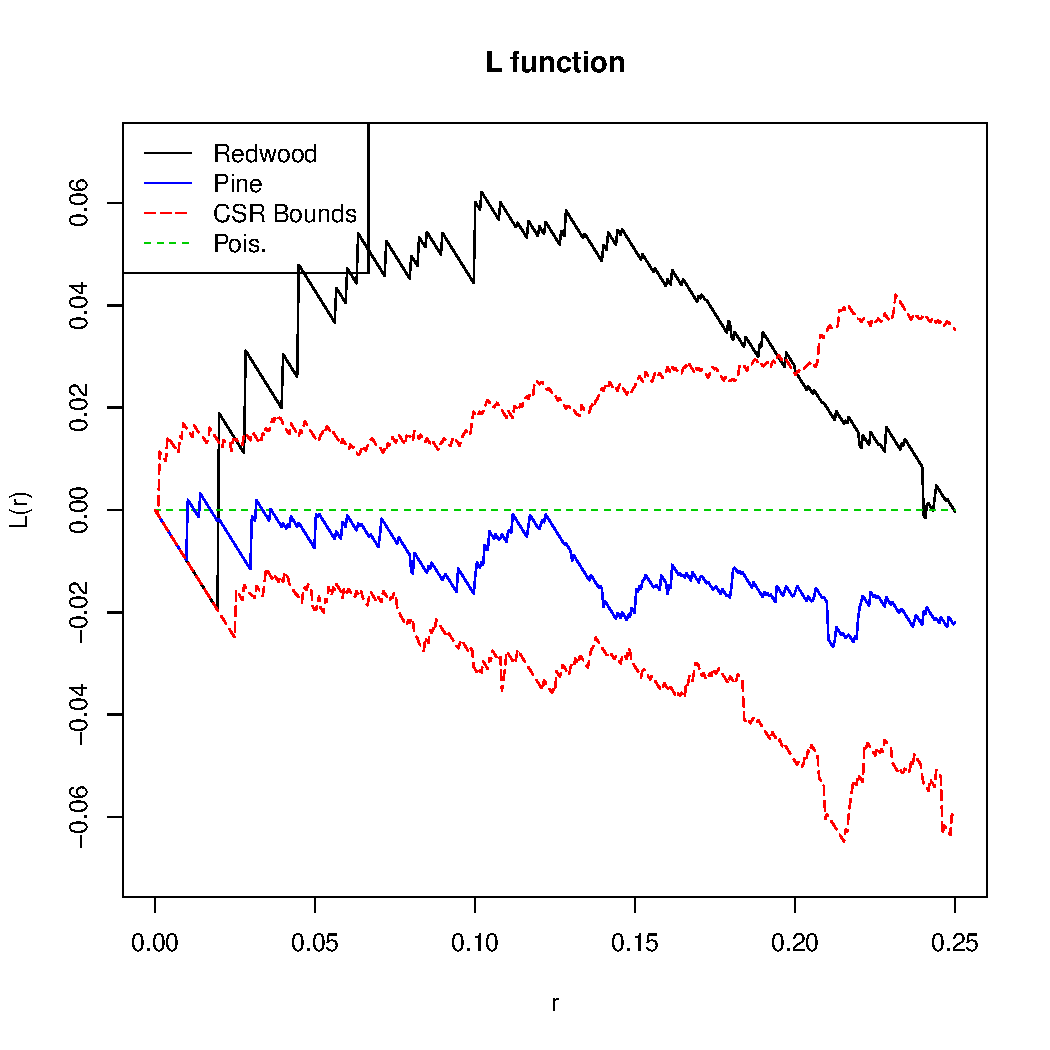
\includegraphics[width=\maxwidth]{figure/Lhat} 

\end{knitrout}
\caption{The $\hat{L}$ plot of the california redwood and Japanese pine data indicating a cluster pattern in the  redwood data and a random pattern in the pine data.  The horizontal green lines shows the expected value for a poisson CSR realization.}
\label{lest}
\end{figure}
\end{document}
